\section{Discussions and Experiments}
\begin{frame}{Part C}
\Large \center{\color{blue}{Discussions and Experiments}}
\end{frame}

\begin{frame}{Datasets for empirical study}
\begin{table}[htbp]
    \centering
    %\caption{Datasets for empirical study} \label{table:dataset}
    \begin{tabular}{|r|r|r|r|r|r}
        \hline
        Dataset & Training($n$) & Test & Features ($d$) & Sparsity($\frac{\nnz}{nd}$) \\
        \hline
        rcv1      & 20,242 & 677,399 & 47,236 & 0.16\% \\
        \hline
        astro-ph       & 29,882  & 32,487    & 99,757 & 0.08\% \\
        \hline
    \end{tabular}
\end{table}
\begin{itemize}
\item \textbf{rcv1} is a corpus from Reuters news stories.
\item \textbf{astro-ph} is astronomy data.
\end{itemize}
\end{frame}

\begin{frame}{Cost per epoch and properties of algorithms}
\begin{table}[htbp]
    \centering
    \label{table:compcost}
    \begin{tabular}{|r|r|r|r|r|}
        \hline
        \textsc{Algorithm} & cost of an epoch & non-uniform & adaptive \\ 
        \hline
        NonUnifSGD & $\nnz$ & \cmark & \xmark  \\
        NonUnifSDCA & $\nnz$ & \cmark & \xmark \\
        AdaSGD & $(k+1)\nnz$ & \cmark & \cmark \\
        AdaSVRG & $nd+k\nnz$  & \cmark & \cmark \\
        AdaSDCA & $(k+1)\nnz$  & \cmark & \cmark \\
        AdaSDCAS & $(k+1)\nnz$  & \cmark & \cmark \\
        AdaGrad (by Duchi) & $2nd$ & \xmark & \xmark \\
        AdaSDCA (by Csiba) & $n\nnz$  & \cmark & \cmark \\
        AdaSDCA+ (by Csiba) & $2\nnz$ & \cmark & \cmark \\
        \hline
    \end{tabular}
\end{table}
\end{frame}

\begin{frame}{Test Error with Different Values of $\lambda$}
\begin{table}[htbp]
    \centering
    \begin{tabular}{|r|r|r|r|r|r|r|}
        \hline
        \texttt{rcv1} & 1e-2 & 5e-3 & \textbf{1e-3} & 5e-4 & 1e-4\\
        \hline
        Test Error & 0.05160 & 0.04833 & \textbf{0.04713} & 0.04913 & 0.05693 \\
        \hline
    \end{tabular}
    \begin{tabular}{|r|r|r|r|r|r|r|}
        \hline
         \texttt{astro-ph} & 1e-2 & 5e-3 & \textbf{1e-3} & 5e-4 & 1e-4 \\
        \hline
        Test Error & 0.04103 & 0.03715 & \textbf{0.03441} & 0.03586 & 0.04371 \\
        \hline
    \end{tabular}
\end{table}
\end{frame}

\begin{frame}{Verifying the Convergence of Duality Gap}
\begin{table}[htbp]
    \centering
    \caption{Average duality gap at different epochs for $\lambda = 0.001$} 
    \label{table:covdual1}
    \begin{tabular}{|r|r|r|}
        \hline
        \#epoch & duality gap on \texttt{rcv1} & duality gap on \texttt{astro-ph} \\ 
        \hline
        1 & 0.0863765 & 0.0883917\\
        3 & 0.0105347 & 6.13163e-03 \\
        10 & 1.7485e-04 & 3.93673e-05 \\
        20 & 2.21547e-05 & 6.24779e-07 \\
        50 & 3.12797e-06 & 6.7474e-10\\
        100 & 5.47897e-07 & 1.43083e-12 \\
        \hline
    \end{tabular}
\end{table}
\end{frame}

\begin{frame}{Performance Metrics}
\begin{definition}\label{def:psds}
The \textbf{primal sub-optimality} of algorithm is defined as $P(\wv(\alphav)) - P(\wv^*)$. 
\end{definition}
\begin{definition}
\textbf{Test error} is the error rate on test dataset.
\end{definition}
\end{frame}

\begin{frame}{Performance of Two Updating Algorithms}
\begin{figure}[htbp]
\begin{tabular}{ll}
    \centering
        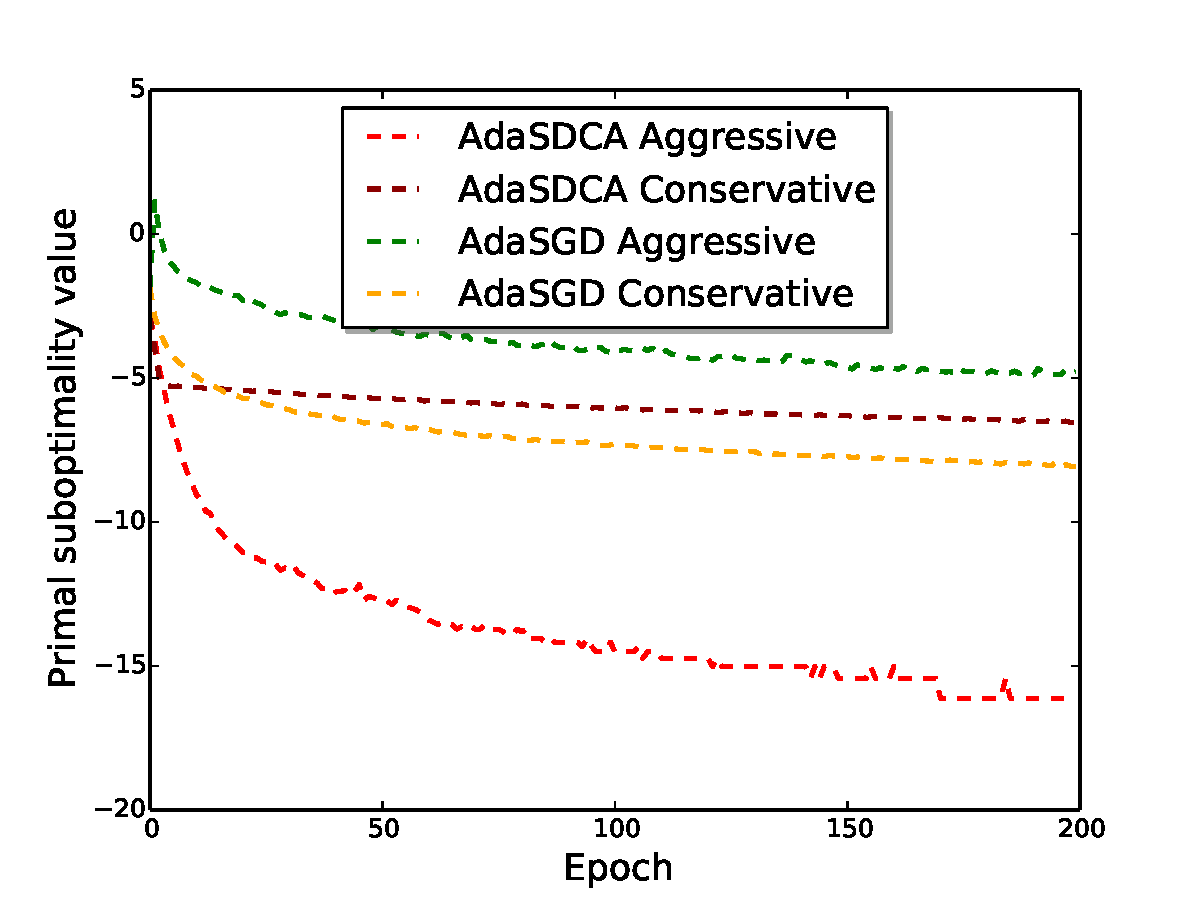
\includegraphics[width=0.5\textwidth]{images/two_updates_obej.pdf} &
        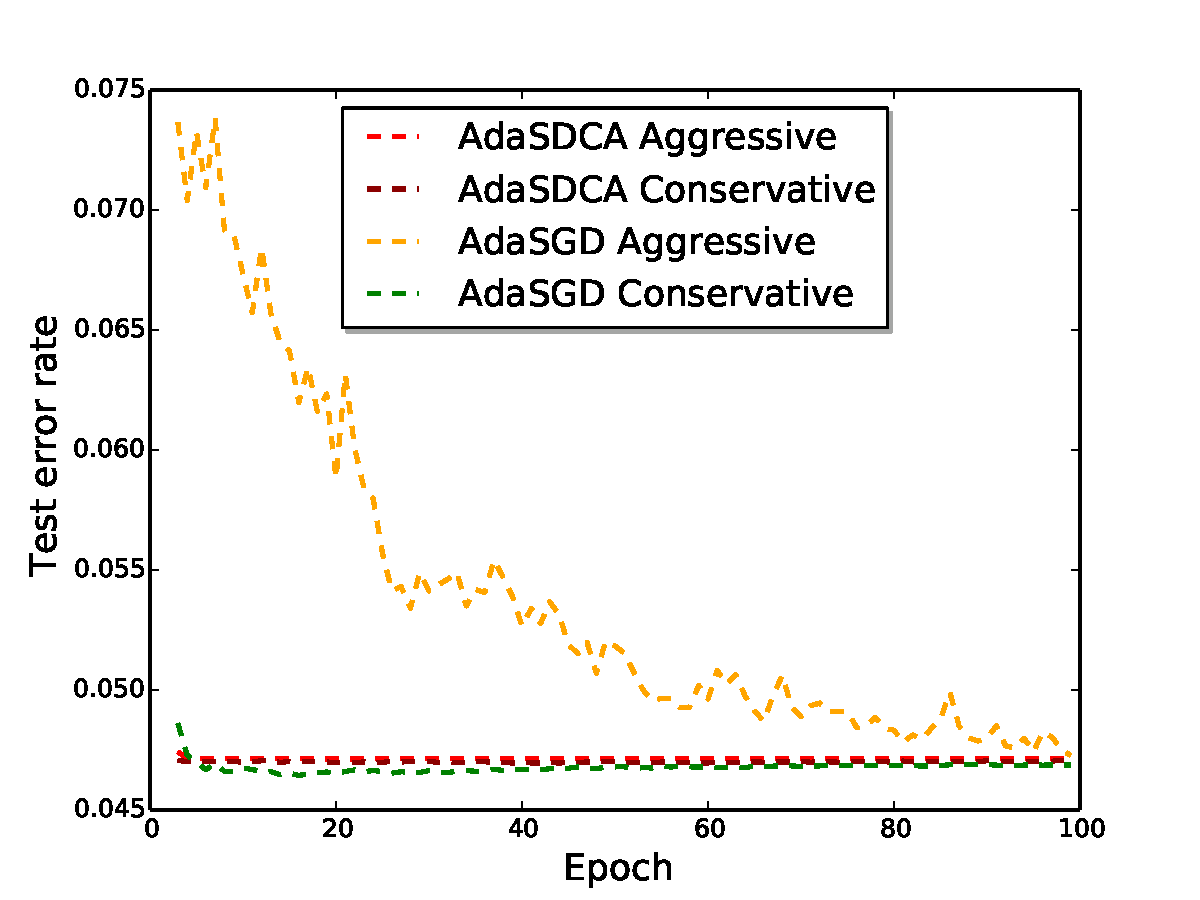
\includegraphics[width=0.5\textwidth]{images/two_updates_terror.pdf}
\end{tabular}
    \caption{Comparison of two updating algorithms for AdaSGD and AdaSDCA on \texttt{rcv1}}
    \label{fig:two_updates}
\end{figure}
\end{frame}

\begin{frame}{Different Adaptive Strategies for AdaSDCA}
\begin{figure}[htbp]
\begin{tabular}{ll}
    \centering
        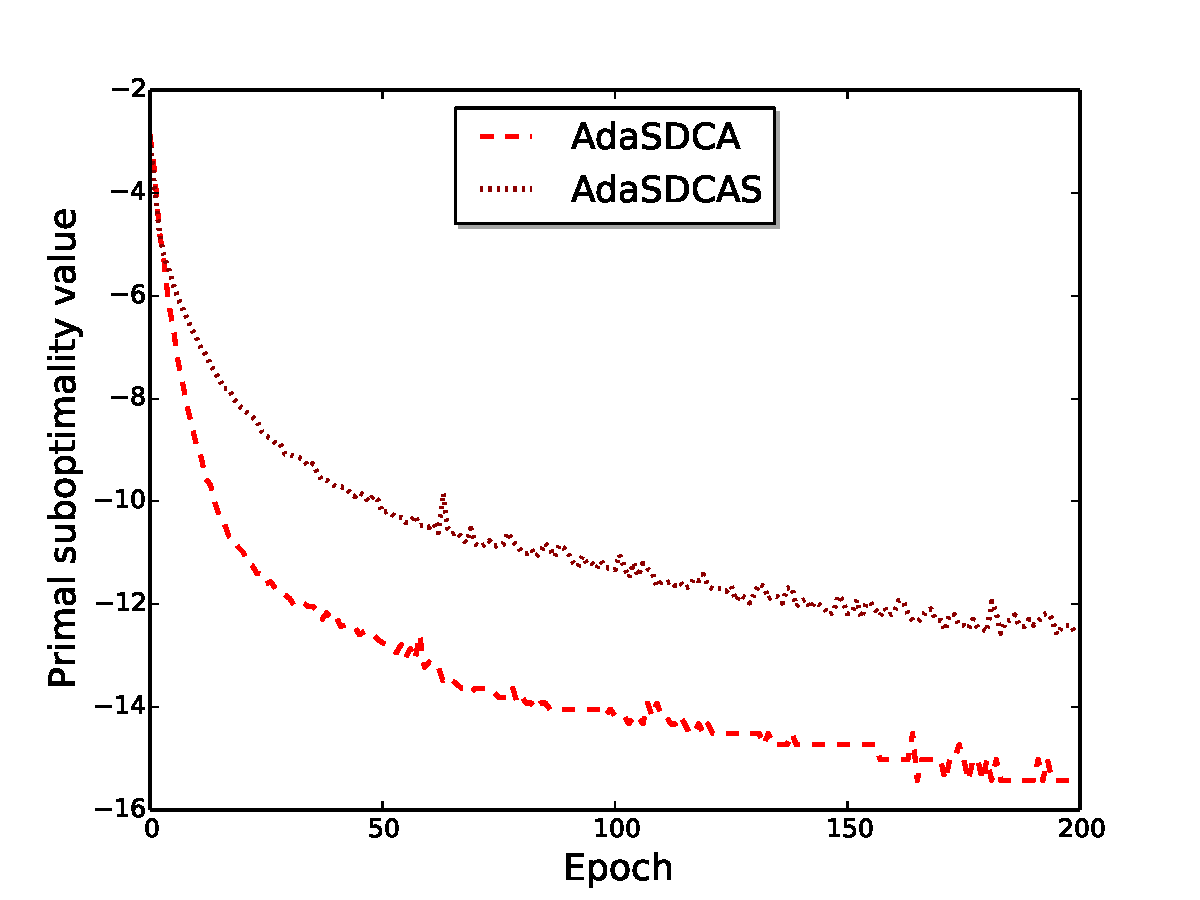
\includegraphics[width=0.5\textwidth]{images/two_strategy_SDCA_obej.pdf} &
        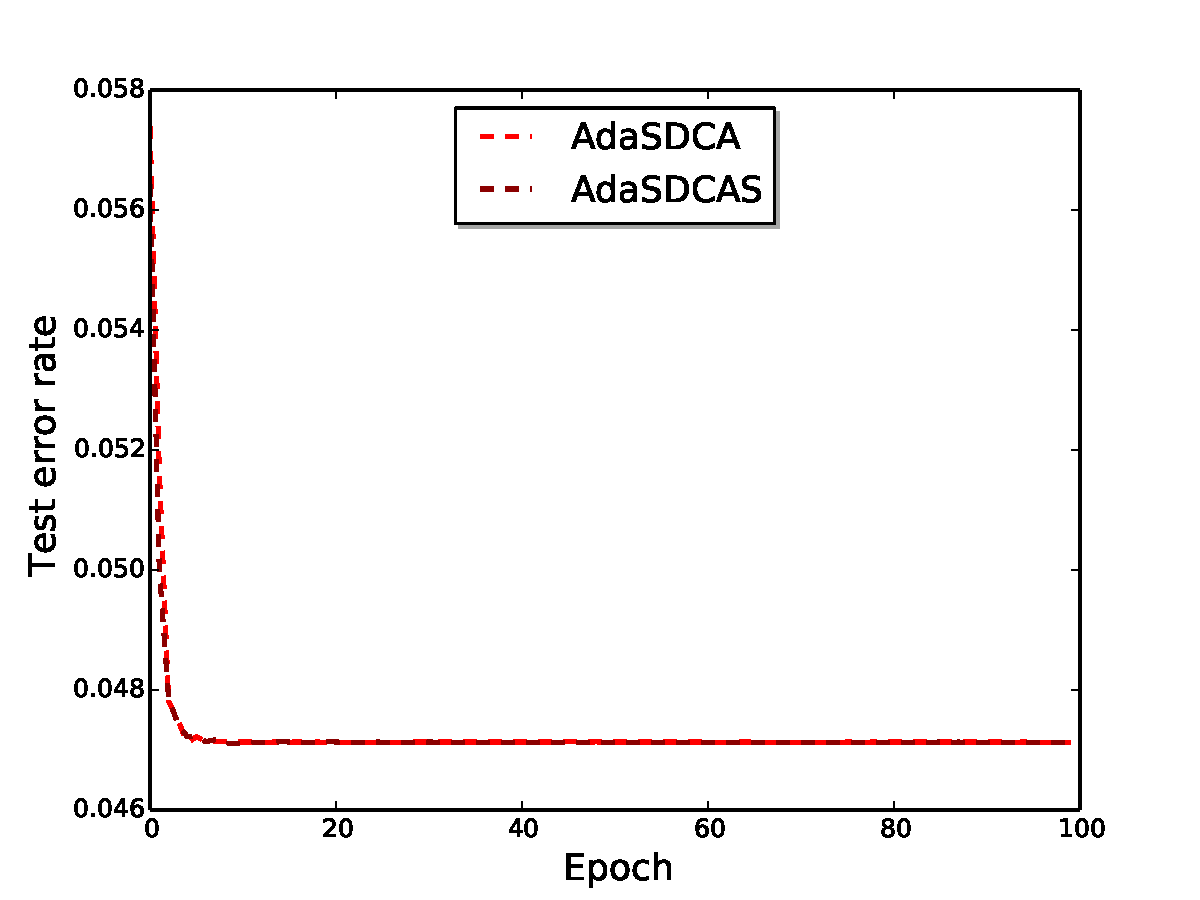
\includegraphics[width=0.5\textwidth]{images/two_strategy_SDCA_terror.pdf}
 \end{tabular}
    \caption{Comparison of AdaSDCA and AdaSDCAS on \texttt{rcv1}}
    \label{fig:sgd_on_sdca}
\end{figure}
\end{frame}

\begin{frame}{Comparison of Average Time}
\begin{table}[htbp]
    \centering
    \caption{Detailed training time and total running time per epoch}
    \label{table:rcv1_time}
    \begin{tabular}{|r|r|r|}
        \hline 
        rcv1 & Training time(s) & Total running time(s) \\
        \hline
        AdaSGD & 0.04765 & 0.2059 \\
        \hline
        AdaSDCA & 0.05042 & 0.2064 \\
        \hline
        NonUnifSGD & 0.04244 & 0.1988 \\
        \hline
        NonUnifSDCA  & 0.04716 & 0.2037 \\
	\hline
    \end{tabular}
    \label{table:astro-ph_time}
    \begin{tabular}{|r|r|r|}
        \hline 
        astro-ph &  Training time(s) & Total running time(s) \\
        \hline
        AdaSGD & 0.07236 & 0.1363 \\
        \hline
        AdaSDCA & 0.07050 & 0.1343 \\
        \hline
        NonUnifSGD & 0.06284 & 0.1259 \\
        \hline
        NonUnifSDCA  & 0.07054 & 0.1339 \\
        \hline
    \end{tabular}
\end{table}
\end{frame}

\begin{frame}{Comparison of Adaptive Algorithms}
\begin{figure}[htbp]
\begin{tabular}{ll}
    \centering
        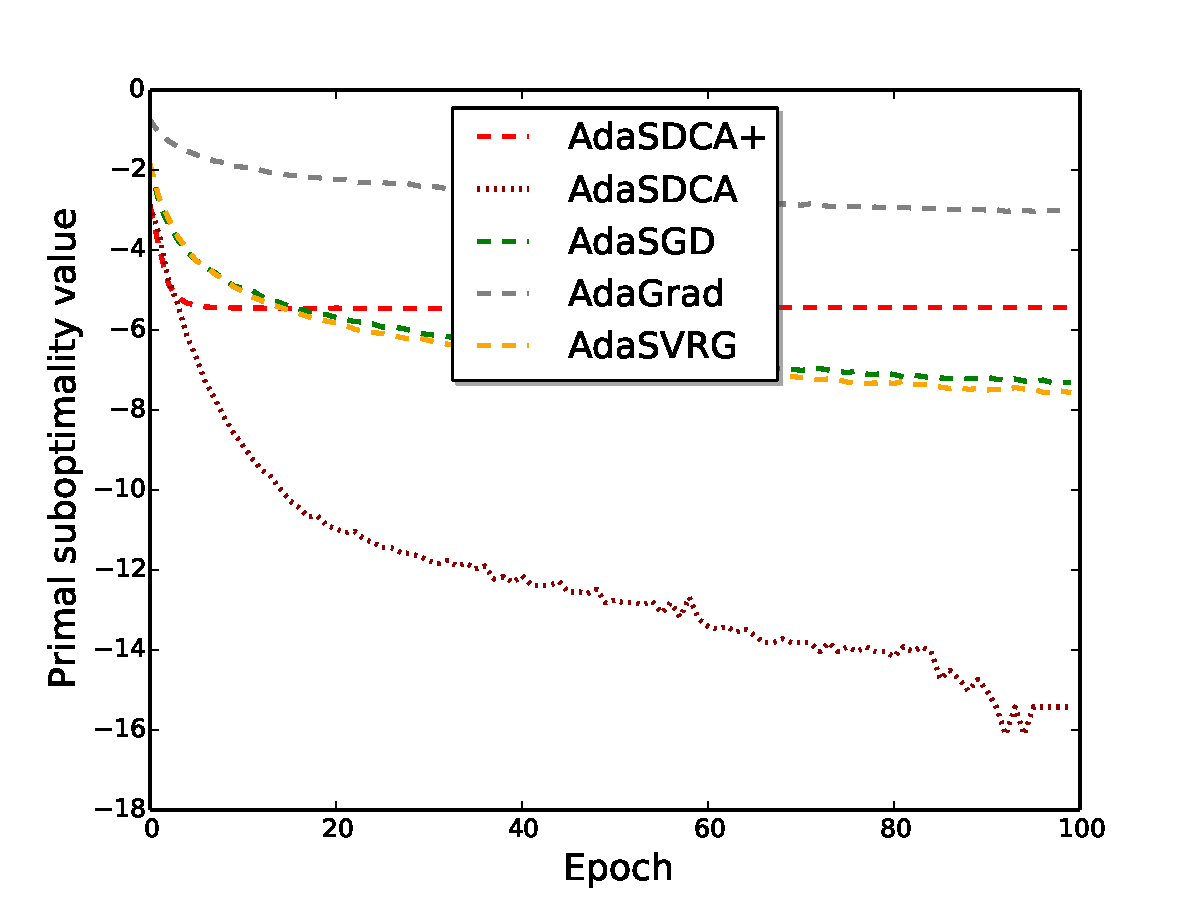
\includegraphics[width=0.5\textwidth]{images/comp_adas_obej.pdf} &
        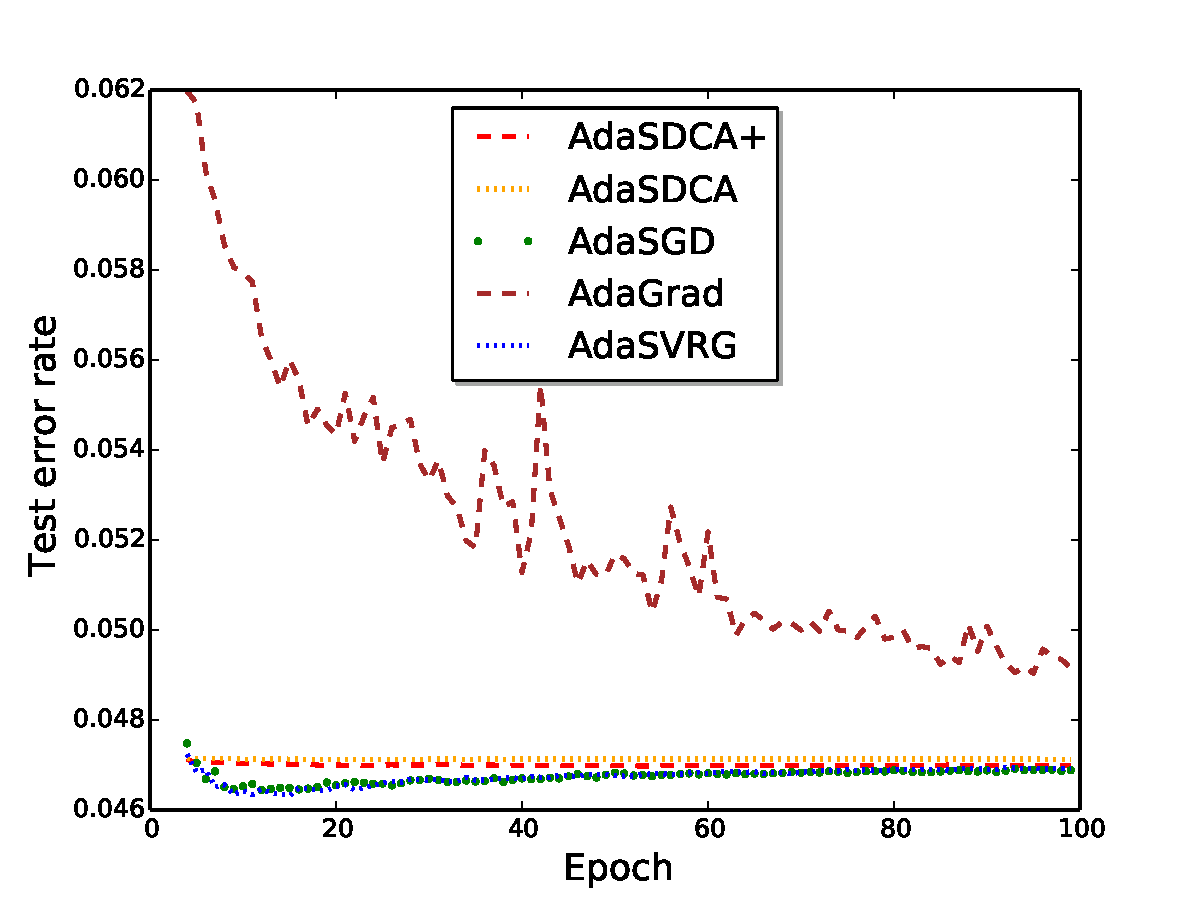
\includegraphics[width=0.5\textwidth]{images/comp_adas_terror.pdf}
        \end{tabular}
    \caption{Comparison of five adaptive algorithms on \texttt{rcv1}} 
    \label{fig:ada_all1}
\end{figure}
\end{frame}

\begin{frame}{Comparison of Adaptive Algorithms cont.}
\begin{figure}[htbp]
\begin{tabular}{ll}
    \centering
        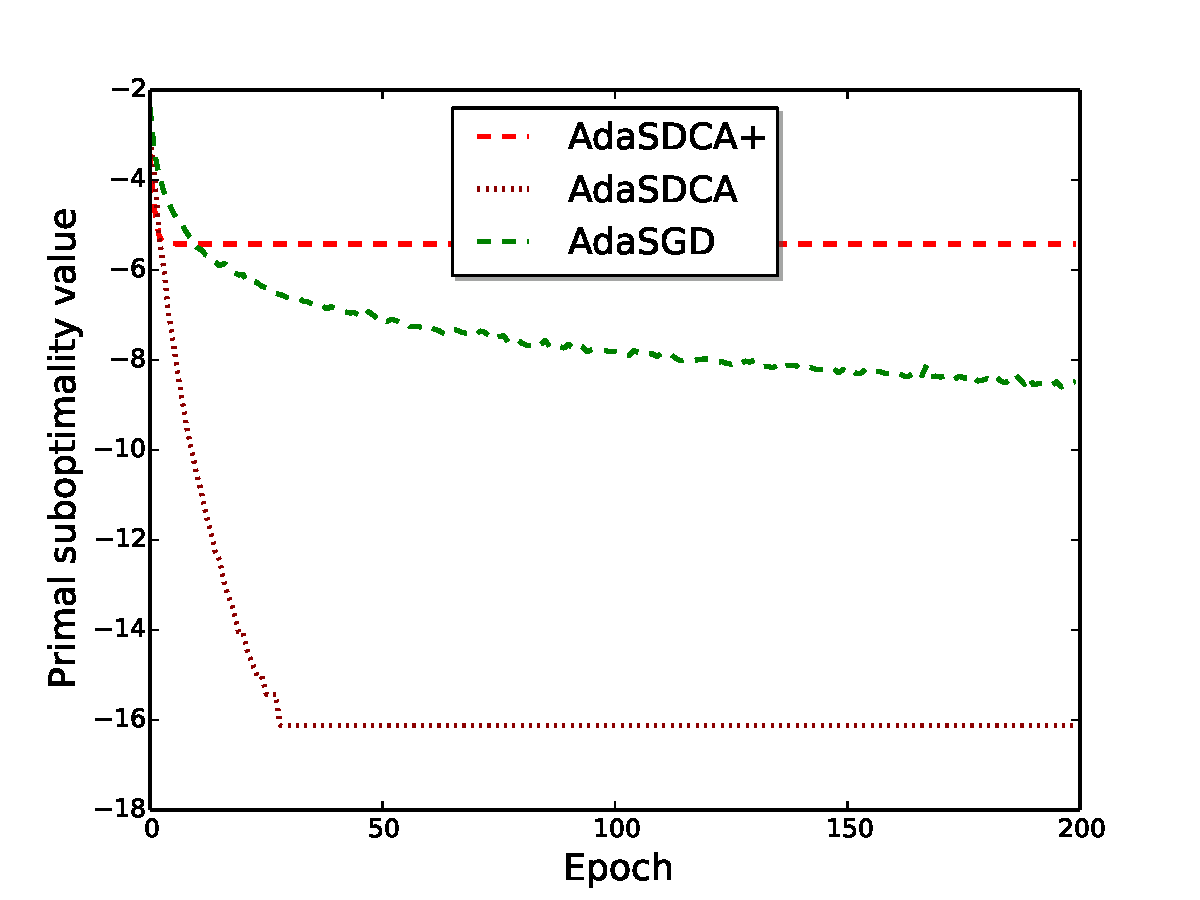
\includegraphics[width=0.5\textwidth]{images/comp_adas_obej_astro.pdf} &
        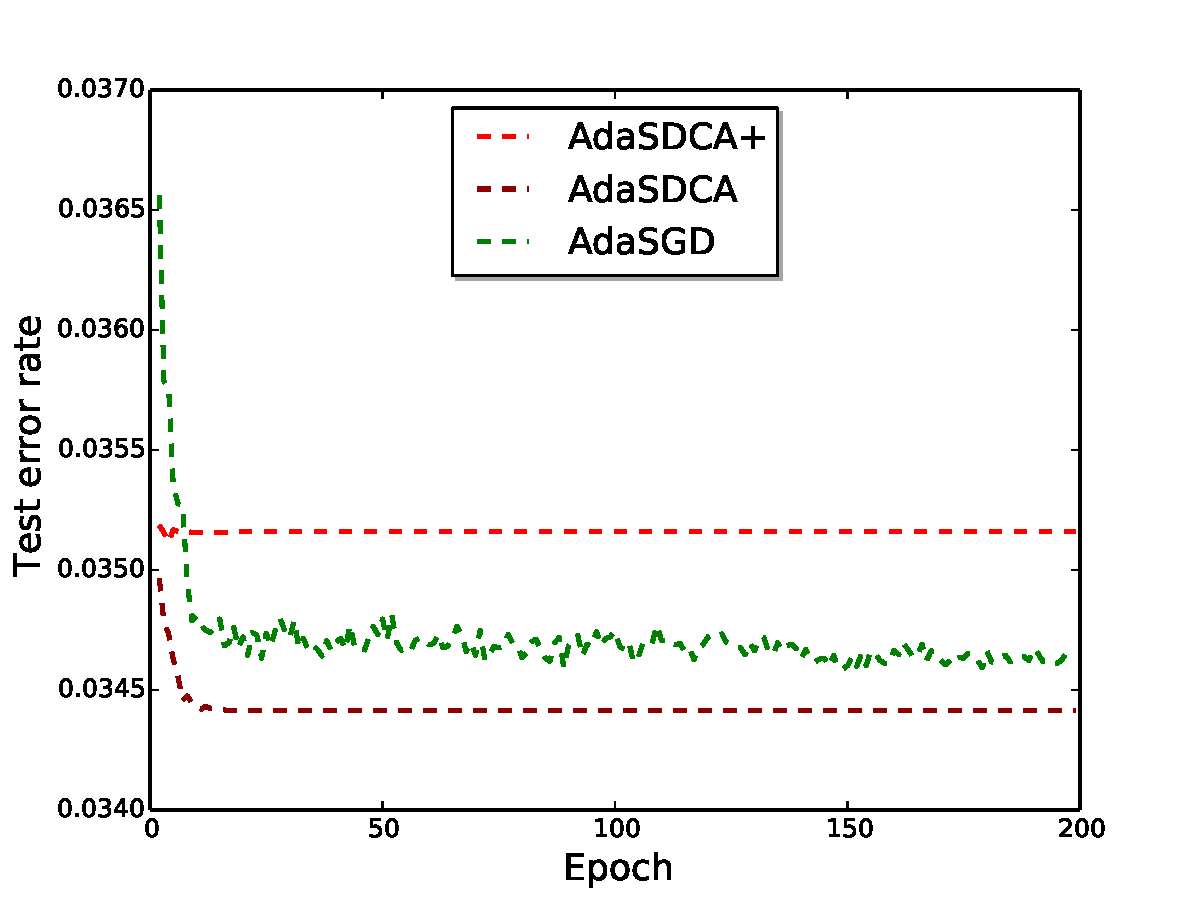
\includegraphics[width=0.5\textwidth]{images/comp_adas_terror_astro.pdf}
        \end{tabular}
    \caption{Comparison of three adaptive algorithms on \texttt{astro-ph}} 
    \label{fig:ada_all2}
\end{figure}
\end{frame}

\begin{frame}{Same Level of Optimality}
\begin{table}[htbp]
    \centering
    \caption{The number of epochs taken to reach the same level of optimality}
    \label{table:timetable}
    \begin{tabular}{|r|r|r|r|r|}
        \hline 
        rcv1 & AdaSDCA & NonUnifSDCA & AdaSGD & NonUnifSGD \\
        \hline
        \#epochs & 9 & 35 & 210 & 500 \\         
        \hline
    \end{tabular}
    \begin{tabular}{|r|r|r|r|r|}
        \hline 
        astro-ph & AdaSDCA & NonUnifSDCA & AdaSGD & NonUnifSGD \\
        \hline
        \#epochs & 8 & 28 & 195 & 500 \\         
        \hline
    \end{tabular}    
\end{table}
\end{frame}

\begin{frame}{Comparison of Time}
\begin{figure}[htbp]
\begin{tabular}{ll}
    \centering
        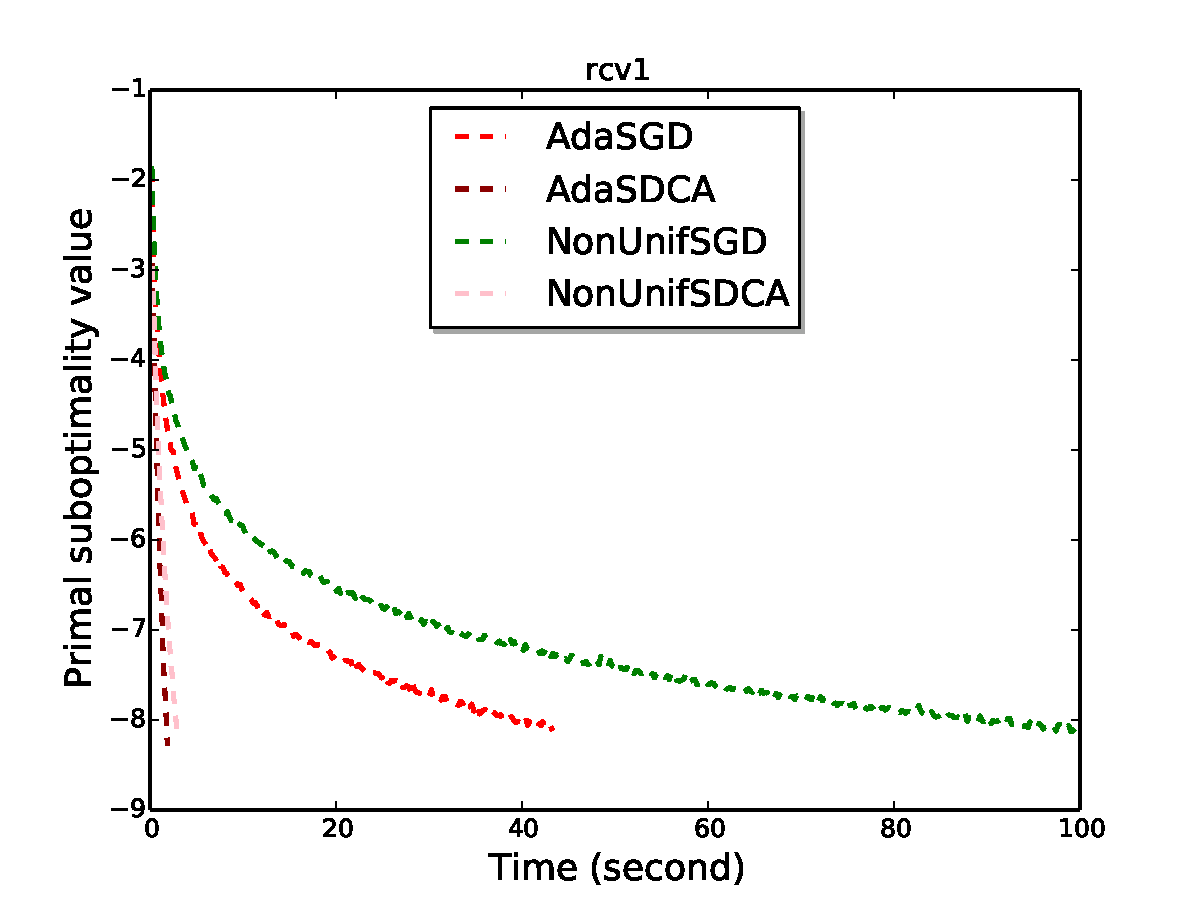
\includegraphics[width=0.5\textwidth]{images/comp_adas_time_rcv1.pdf} &
        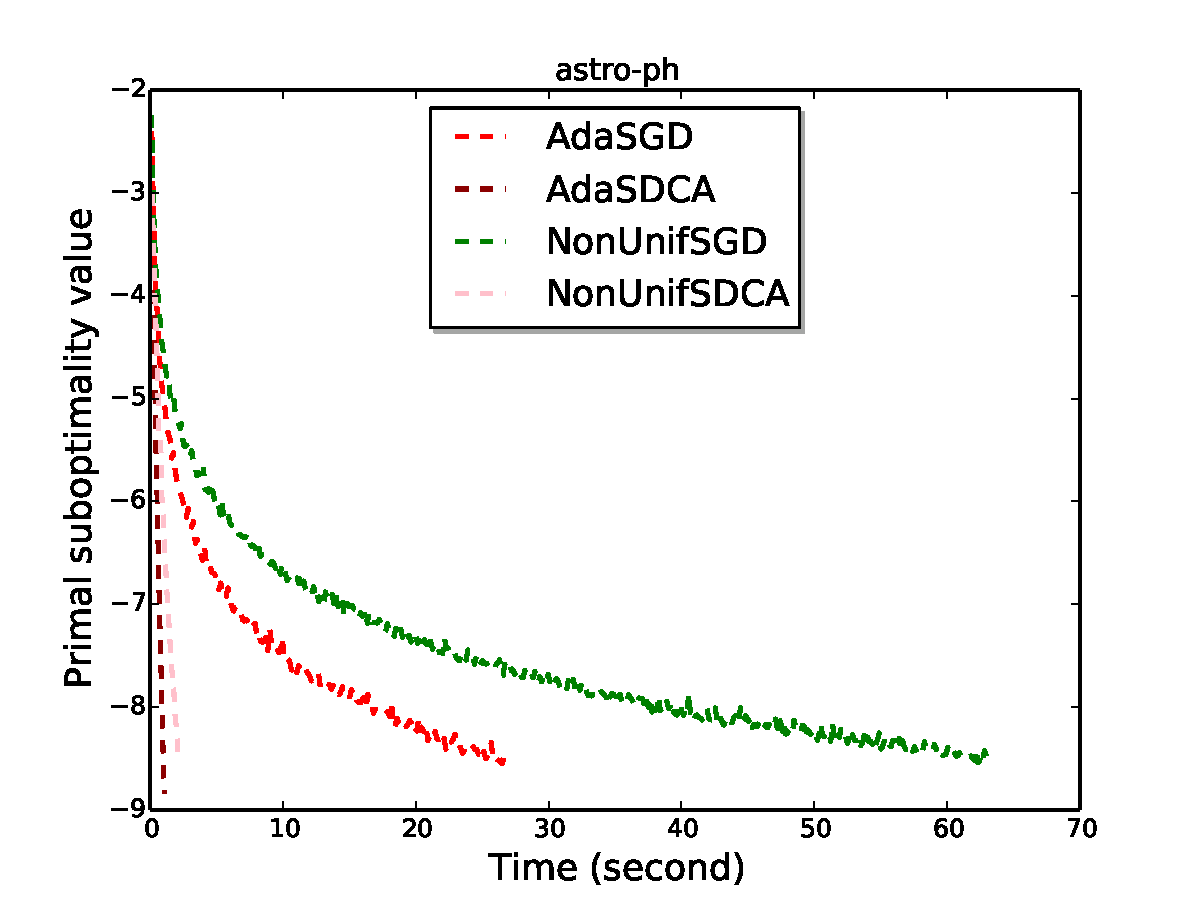
\includegraphics[width=0.5\textwidth]{images/comp_adas_time_astro.pdf}
\end{tabular}
        \caption{Comparison of the total running time to reach the same optimality}
     \label{fig:adatime}
\end{figure}
\end{frame}

\begin{frame}{Comparison of Vector Operation}
\begin{figure}[htbp]
\begin{tabular}{ll}
    \centering
        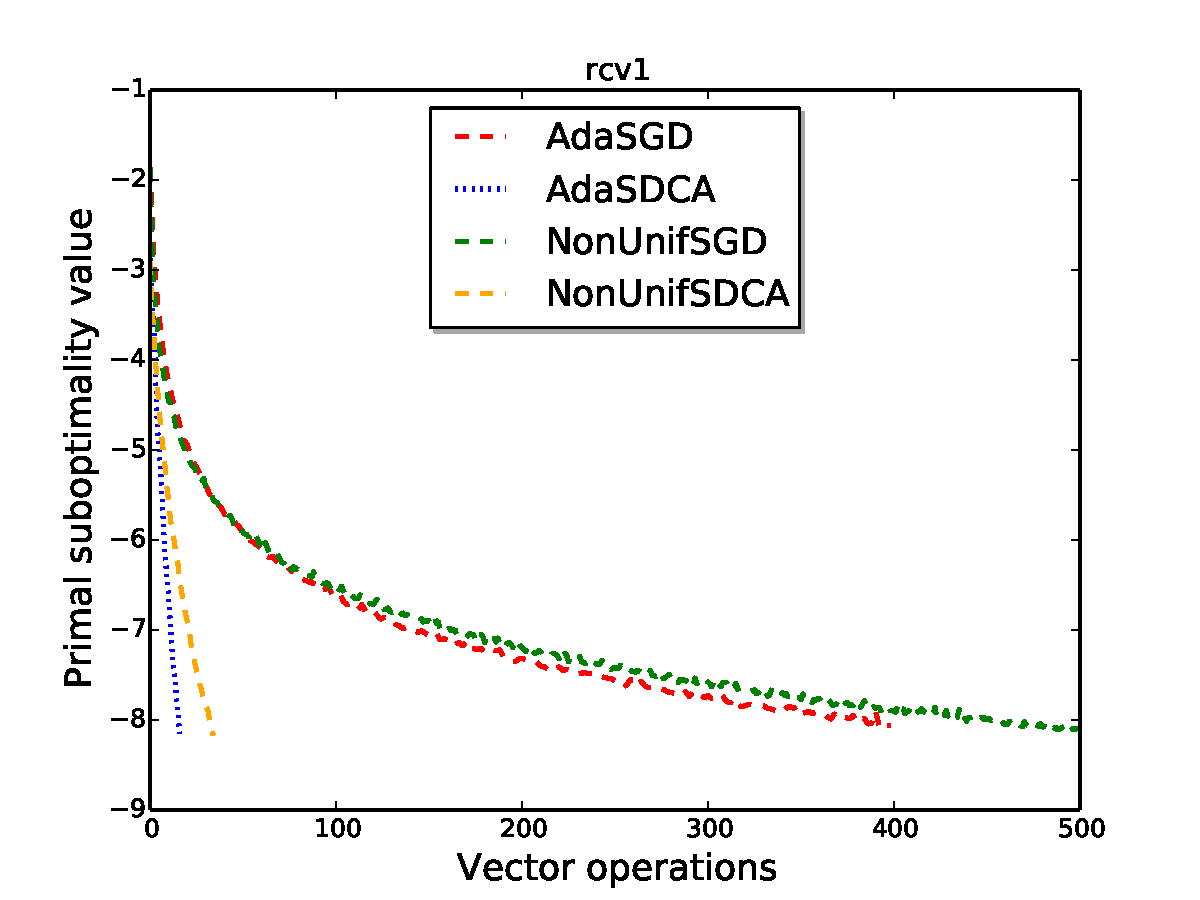
\includegraphics[width=0.5\textwidth]{images/comp_adas_vector_rcv1.pdf} &
        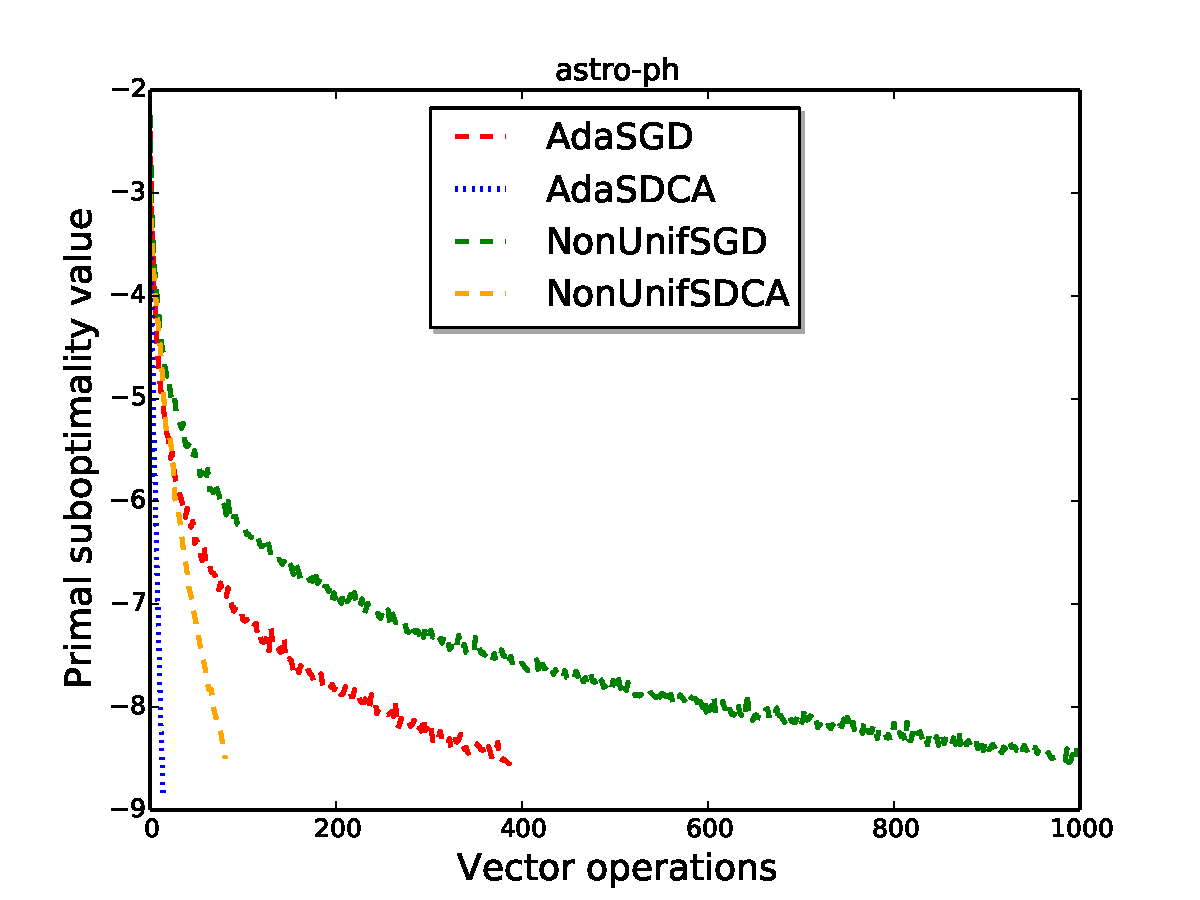
\includegraphics[width=0.5\textwidth]{images/comp_adas_vector_astro.pdf}
\end{tabular}
        \caption{Comparison of the vector operations taken to reach the same optimality}
     \label{fig:vectorop}
\end{figure}
\end{frame}

\begin{frame}{Adaptive vs. Non-Uniform Algorithms}
\begin{figure}[htbp]
\begin{tabular}{ll}
    \centering
        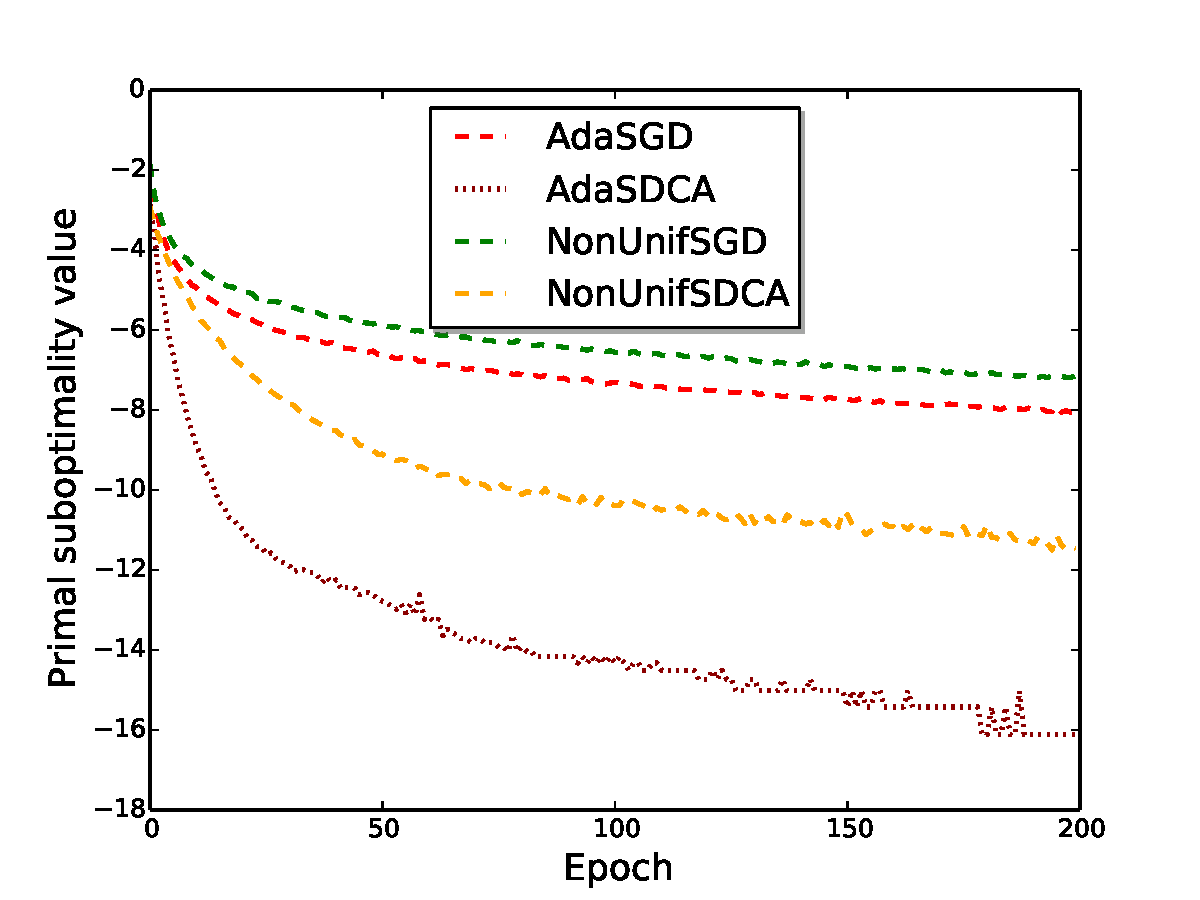
\includegraphics[width=0.5\textwidth]{images/comp_all_obej.pdf} &
        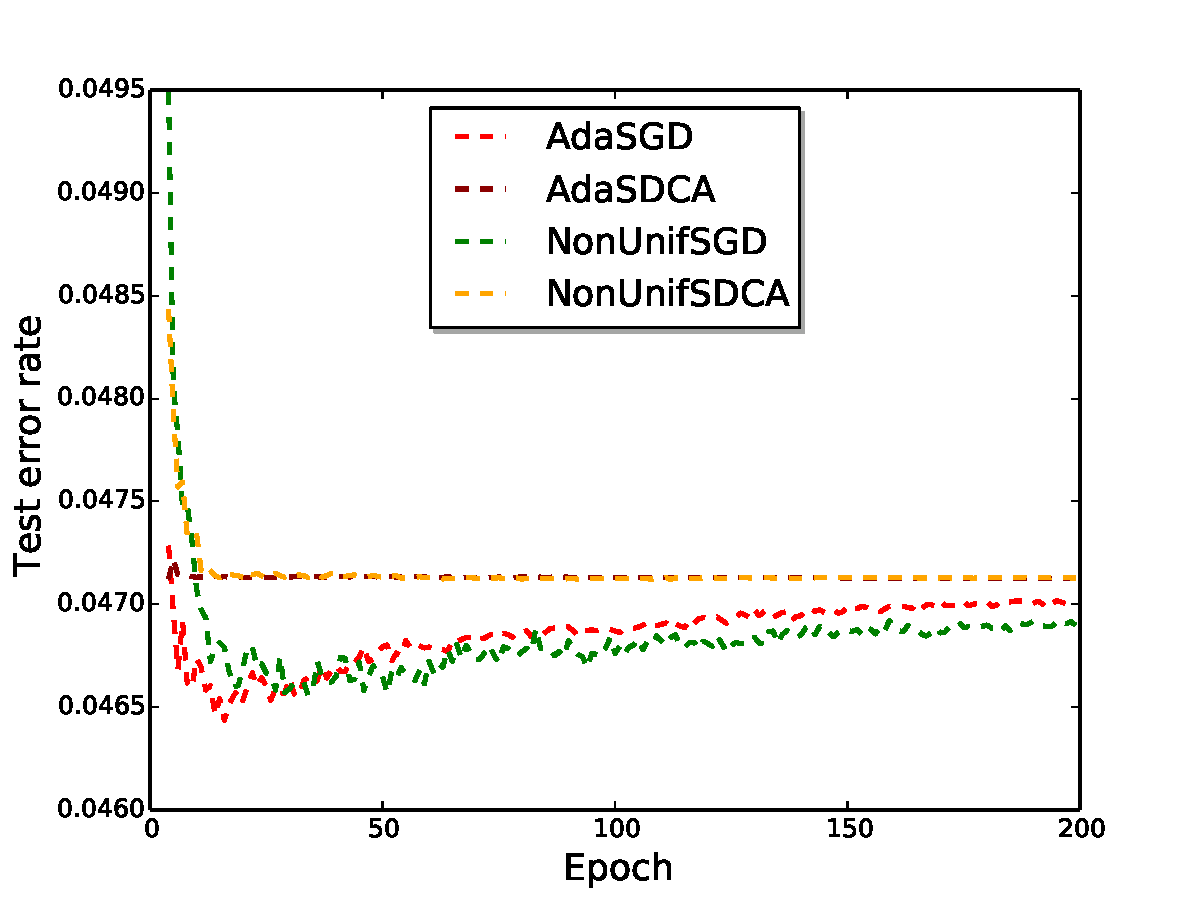
\includegraphics[width=0.5\textwidth]{images/comp_all_terror.pdf}
    \end{tabular}
    \caption{Comparison of adaptive algorithms with non-adaptive algorithms on \texttt{rcv1}} 
    \label{fig:comp_all1}
\end{figure}
\end{frame}

\begin{frame}{Adaptive vs. Non-Uniform Algorithms cont.}
\begin{figure}[htbp]
\begin{tabular}{ll}
    \centering
        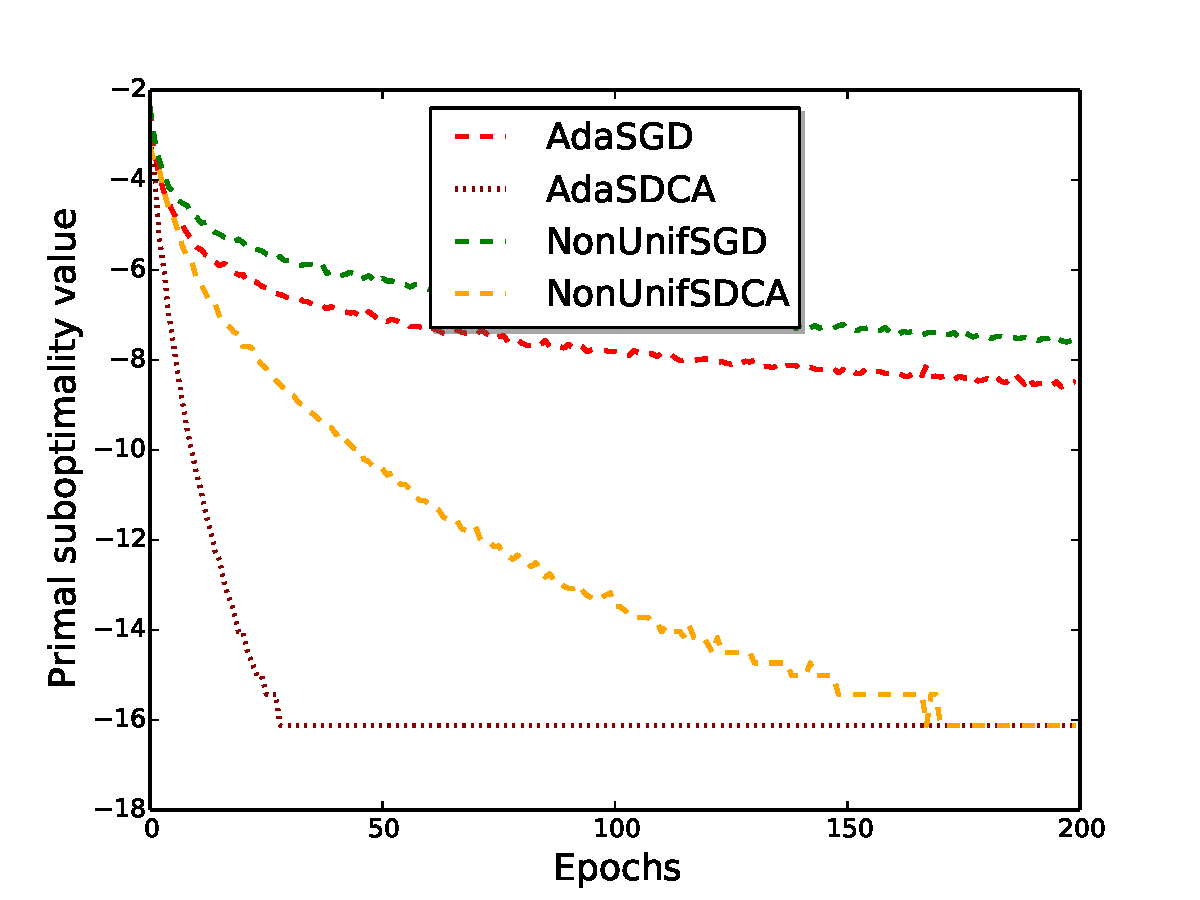
\includegraphics[width=0.5\textwidth]{images/comp_all_obej_astro.pdf} &
        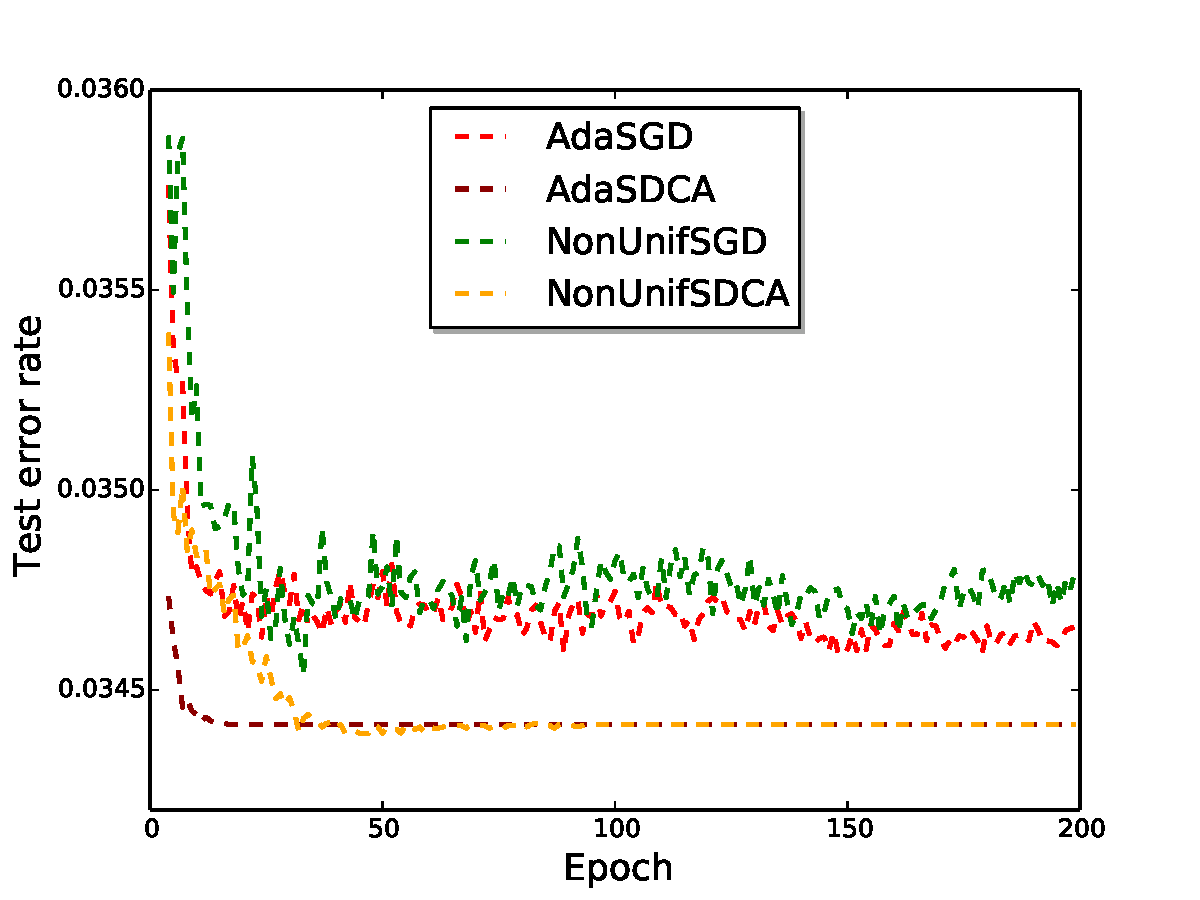
\includegraphics[width=0.5\textwidth]{images/comp_all_terror_astro.pdf}
    \end{tabular}
    \caption{Comparison of adaptive algorithms with non-adaptive algorithms on \texttt{astro-ph}} 
    \label{fig:comp_all2}
\end{figure}
\end{frame}


\begin{frame}{Summary}
\begin{itemize}
	\item We chose $\lambda=0.001$ for both \texttt{rcv1} and \texttt{astro-ph}.
	\item We compare the performance of Conservative Update and Aggressive Update on AdaSGD and AdaSDCA. Conservative Update works better on AdaSGD  while Aggressive Update works better on AdaSDCA.
	\item AdaSDCA (adaptive algorithm with duality gap) performs better than AdaSDCAS (adaptive algorithm with subgradients).
	\item AdaSDCA has the best performance among all the adaptive algorithms (AdaSDCA, AdaSGD, AdaSVRG, AdaGrad and AdaSDCA+) and AdaSGD is the second best.
\end{itemize}
\end{frame}
\begin{frame}{Summary cont.}
\begin{itemize}
	\item AdaSVRG achieves a slightly better performance per epoch than AdaSGD but sacrifices the running time on sparse datasets.
	\item To reach the same optimality given by $500$ epochs run on NonUnifSGD, AdaSGD takes only around $200$ epochs, whereas NonUnifSDCA takes around $30$ which is three times more than AdaSDCA does.
\end{itemize}
\end{frame}

